\begin{figure}[ht]
    \centering
    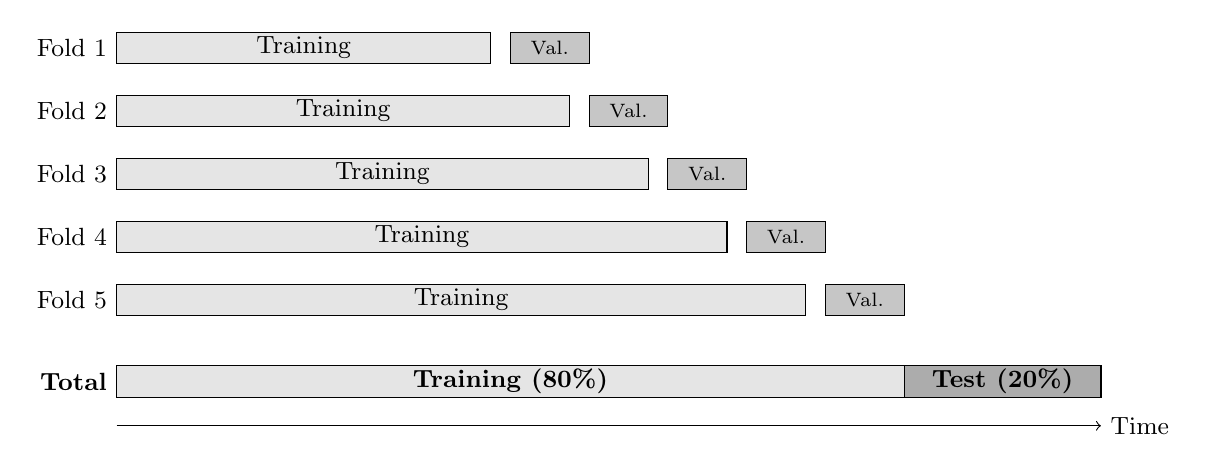
\begin{tikzpicture}[
        x=1.25cm,
        y=0.8cm,
        font=\small
    ]

    % Fold 1
    \node[anchor=east] at (0,0) {Fold 1};
    \draw[fill=gray!20] (0,-0.25) rectangle (3.80,0.25);
    \node at (1.90,0) {Training};
    \draw[fill=gray!45] (4.00,-0.25) rectangle (4.80,0.25);
    \node at (4.40,0) {\scriptsize Val.};

    % Fold 2
    \node[anchor=east] at (0,-1) {Fold 2};
    \draw[fill=gray!20] (0,-1.25) rectangle (4.60,-0.75);
    \node at (2.30,-1) {Training};
    \draw[fill=gray!45] (4.80,-1.25) rectangle (5.60,-0.75);
    \node at (5.20,-1) {\scriptsize Val.};

    % Fold 3
    \node[anchor=east] at (0,-2) {Fold 3};
    \draw[fill=gray!20] (0,-2.25) rectangle (5.40,-1.75);
    \node at (2.70,-2) {Training};
    \draw[fill=gray!45] (5.60,-2.25) rectangle (6.40,-1.75);
    \node at (6.00,-2) {\scriptsize Val.};

    % Fold 4
    \node[anchor=east] at (0,-3) {Fold 4};
    \draw[fill=gray!20] (0,-3.25) rectangle (6.20,-2.75);
    \node at (3.10,-3) {Training};
    \draw[fill=gray!45] (6.40,-3.25) rectangle (7.20,-2.75);
    \node at (6.80,-3) {\scriptsize Val.};

    % Fold 5
    \node[anchor=east] at (0,-4) {Fold 5};
    \draw[fill=gray!20] (0,-4.25) rectangle (7.00,-3.75);
    \node at (3.50,-4) {Training};
    \draw[fill=gray!45] (7.20,-4.25) rectangle (8.00,-3.75);
    \node at (7.60,-4) {\scriptsize Val.};

    % Total split
    \node[anchor=east] at (0,-5.3) {\textbf{Total}};

    \draw[fill=gray!20]
        (0,-5.55) rectangle (8,-5.05);
    \node at (4,-5.3) {\textbf{Training (80\%)}};

    \draw[fill=gray!65]
        (8,-5.55) rectangle (10,-5.05);
    \node at (9,-5.3) {\textbf{Test (20\%)}};

    % Time axis
    \draw[->] (0,-6.0) -- (10,-6.0)
        node[right] {Time};

    \end{tikzpicture}

    \caption{Schematic overview of expanding window \ac{CV} with five folds. The first fold uses about 50\% of the training data for training and each validation set contains about 10\%. Validation sets do not overlap. The 24-hour gap between training and validation is enlarged for visibility.}
    \label{fig:expanding-window-cv}
\end{figure}